\documentclass[border=10pt]{standalone}
\usepackage{tikz,amsmath}
\usetikzlibrary{arrows.meta}

% ========== 配色 ==========
\definecolor{inFill}{RGB}{183,224,177}
\definecolor{inLine}{RGB}{32,102,32}
\definecolor{blFill}{RGB}{214,228,250}
\definecolor{blLine}{RGB}{60,90,170}
\definecolor{orFill}{RGB}{250,224,180}
\definecolor{orLine}{RGB}{190,110,20}
\definecolor{hidFill}{RGB}{199,203,243}
\definecolor{hidLine}{RGB}{52,58,143}
\definecolor{opFill}{RGB}{250,250,250}
\definecolor{opLine}{RGB}{70,70,70}

\begin{document}
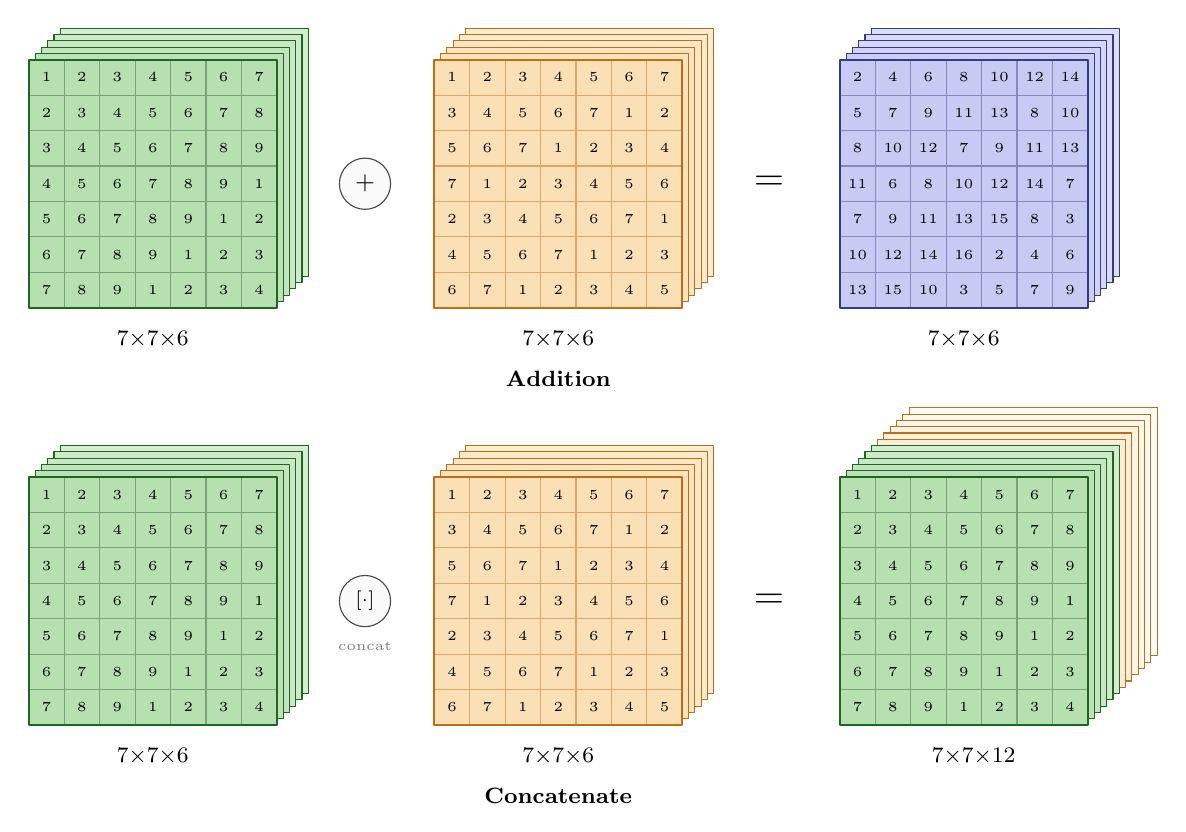
\begin{tikzpicture}[
    font=\small, line join=round,
    every node/.style={inner sep=0pt, outer sep=0pt, align=center},
    add/.style={circle, draw=opLine, fill=opFill, minimum size=.65cm}
  ]

  % ========== 格内数字：#3 = 0(A) / 1(B) / 2(A+B) ==========
  \newcommand{\cellnums}[3]{%
    \foreach \r in {0,...,6} \foreach \c in {0,...,6} {%
      \pgfmathtruncatemacro{\va}{mod(\r+\c,9)+1}
      \pgfmathtruncatemacro{\vb}{mod(2*\r+\c,7)+1}
      \ifcase#3 \def\vv{\va}\or\def\vv{\vb}\or\pgfmathtruncatemacro{\vv}{\va+\vb}\fi
      \node[font=\tiny] at ({#1+0.45*\c+0.225},{#2+0.45*(6-\r)+0.225}) {\vv};
    }%
  }

  % ========== 带数字的特征图堆叠（★ 背片偏移 0.08）：#5 = 0无/1=A/2=B/3=A+B ==========
  \newcommand{\fmap}[5]{%
    \pgfmathtruncatemacro{\Nb}{#4-1}
    \foreach \k in {\Nb,...,1}{%
      \pgfmathtruncatemacro{\op}{100-8*\k}
      \fill[#3Fill!\op, draw=#3Line, line width=.4pt]
            ({#1+0.08*\k},{#2+0.08*\k}) rectangle ++(3.15,3.15);
    }
    \fill[#3Fill] (#1,#2) rectangle ++(3.15,3.15);
    \draw[step=.45, #3Line!60, line width=.4pt, shift={(#1,#2)}] (0,0) grid (3.15,3.15);
    \draw[#3Line, thick] (#1,#2) rectangle ++(3.15,3.15);
    \ifnum#5=1 \cellnums{#1}{#2}{0}\fi
    \ifnum#5=2 \cellnums{#1}{#2}{1}\fi
    \ifnum#5=3 \cellnums{#1}{#2}{2}\fi
  }

  % ========== concat 结果：绿6片+橙6片=12片，正面保留 A 的数字（★ 后半部改橙色） ==========
  \newcommand{\catstack}[2]{%
    \foreach \k in {11,...,1}{%
      \ifnum\k>5 \def\cc{or}\else \def\cc{in}\fi
      \pgfmathtruncatemacro{\op}{100-8*\k}
      \fill[\cc Fill!\op, draw=\cc Line, line width=.4pt]
            ({#1+0.08*\k},{#2+0.08*\k}) rectangle ++(3.15,3.15);
    }
    \fill[inFill] (#1,#2) rectangle ++(3.15,3.15);
    \draw[step=.45, inLine!60, line width=.4pt, shift={(#1,#2)}] (0,0) grid (3.15,3.15);
    \draw[inLine, thick] (#1,#2) rectangle ++(3.15,3.15);
    \cellnums{#1}{#2}{0}
  }

  % ================= 上行：element-wise add（7x7x6 + 7x7x6 = 7x7x6） =================
  \fmap{0}{0}{in}{6}{1}
  \node[add] at (4.27,1.575) {+};
  \fmap{5.15}{0}{or}{6}{2}
  \node[font=\Large] at (9.4,1.575) {$=$};
  \fmap{10.3}{0}{hid}{6}{3}
  \node[font=\footnotesize] at (1.575,-0.4)  {7$\times$7$\times$6};
  \node[font=\footnotesize] at (6.725,-0.4) {7$\times$7$\times$6};
  \node[font=\footnotesize] at (11.875,-0.4){7$\times$7$\times$6};
  \node[font=\footnotesize\bfseries] at (6.725,-0.9){Addition};

  % ================= 下行：concat（7x7x6 , 7x7x6 = 7x7x12）★ 间隙收紧 =================
  \fmap{0}{-5.3}{in}{6}{1}
  \node[add, font=\scriptsize] at (4.27,-3.725) {$[\cdot]$};
  \node[font=\tiny, text=gray] at (4.27,-4.3) {concat};
  \fmap{5.15}{-5.3}{or}{6}{2}
  \node[font=\Large] at (9.4,-3.725) {$=$};
  \catstack{10.3}{-5.3}
  \node[font=\footnotesize] at (1.575,-5.7)  {7$\times$7$\times$6};
  \node[font=\footnotesize] at (6.725,-5.7) {7$\times$7$\times$6};
  \node[font=\footnotesize] at (12.0,-5.7)  {7$\times$7$\times$12};
  \node[font=\footnotesize\bfseries] at (6.725,-6.2) {Concatenate};

\end{tikzpicture}
\end{document}